\documentclass[aspectratio=169,10pt]{beamer}

%%%%%%%%%%%%%%%%% Theme %%%%%%%%%%%%%%%%%

\usetheme[language=ger,flag=pride]{cogsys}

%%%%%%%%%%%%%%%%% Packages (optional) %%%%%%%%%%%%%%%%%

\usepackage[ngerman]{babel}
\usepackage{csquotes}
\usepackage{graphicx}                               % Figures
% \usepackage{booktabs}                               % Better tables
\usepackage{tikz}

% Literature: needed for \framecite / \framebib (full references on the slide)
\usepackage[style=apa,backend=biber]{biblatex}
\addbibresource{refs.bib}

%%%%%%%%%%%%%%%%% Commands/Makros %%%%%%%%%%%%%%%%%

\newcommand{\urllink}[2]{\href{#1}{\textcolor{blue!60}{\underline{#2}}}}

%%%%%%%%%%%%%%%%% Metadata %%%%%%%%%%%%%%%%%

\title{Natürliche Sprachverarbeitung mit KI}
% \subtitle{@@SUBTITLE@@}
\author[Voigt, Langer]{Erik Voigt, Johannes Langer}
\course[SMW Bundeskonferenz 2026]{Natürliche Sprachverarbeitung mit KI}
% \semester{@@SEMESTER@@}
% \lecturenumber{@@LECTURENUM@@}
\date{14/15. Nov 2026}

%%%%%%%%%%%%%%%%% Document %%%%%%%%%%%%%%%%%

\begin{document}

\begin{frame}
    \titlepage
\end{frame}

\begin{frame}[c]{Gliederung}
    \small
    \tableofcontents
\end{frame}

%%%%%%%%%%%%%%%%% Was Ist Natürliche Sprachverarbeitung? %%%%%%%%%%%%%%%%%
\section{Natürliche Sprachverarbeitung: Grundlagen}

\begin{frame}{Natürliche Sprachverarbeitung}

\end{frame}

\begin{frame}{Maschinelles Lernen}

\end{frame}

\begin{frame}{Neuronale Netze}

\end{frame}

%%%%%%%%%%%%%%%%% Probabilistische Sprachmodelle %%%%%%%%%%%%%%%%%
\section{Probabilistische Sprachmodelle}

\subsection{Definition und Begriffe}

\begin{frame}{Probabilistische Sprachmodelle}{Definition}
    \begin{definition}[Probabilistisches Sprachmodell]
        Ein \textbf{statistisches} oder \textbf{probabilistisches Sprachmodell} kann durch die \emph{bedingte Wahrscheinlichkeit} des nächsten Wortes, gegeben aller vorherigen Worte repräsentiert werden. Dann ist die Wahrscheinlichkeit einer Wortfolge
        \begin{equation*}
            \hat{P}(w_1, \dots, w_T)=\prod_{i=1}^{T}\hat{P}(w_i~\vert~w_1,\dots,w_{i-1}).
        \end{equation*}
    \end{definition}
    \framebib{bengioNeuralProbabilisticLanguage2003}
\end{frame}

\begin{frame}{Begriffe}
    \begin{definition}[Token]
        Ein \textbf{Token} ist die kleinste diskrete Einheit in der Sprachmodellierung. Token können Zeichen, Wortteile, Wörter, oder sogar ganze Sätze sein.
    \end{definition}

    \begin{definition}[Vokabular]
        Das \textbf{Vokabular} $V$ ist die Menge der einzigartigen \emph{Token} bei der Sprachmodellierung. Die Größe des Vokabulars $\lvert V\rvert$ beschreibt den \emph{Zustandsraum} des Modells. Token, die nicht im Vokabular enthalten sind, kennt das Modell nicht, und können nicht verarbeitet werden.
    \end{definition}

    % TODO: Wollen wir das drin haben? Ist ja eigentlich ein Mix...
    % \footnotetext{Wortteile haben sich in der Praxis als die effektivste Tokenebene herausgestellt.}
\end{frame}

\subsection{N-Gram Modelle}

\begin{frame}[essential]{N-Gram Modelle}
    In der Praxis ist die Berechnung beliebig langer Token-Sequenzen unmöglich. Ein \emph{N-Gram Sprachmodell} trifft die \emph{Markov-Annahme} $N$-ter Ordnung: Die Wahrscheinlichkeit des Tokens $i$ hängt nur von den vorherigen $N-1$ Token ab. $N$ wird auch als \emph{Ordnung} des N-Gram Modells bezeichnet.

    \begin{definition}[N-Gram Sprachmodell]
        Ein \textbf{N-Gram Sprachmodell} ist ein \emph{probabilistisches Sprachmodell} unter der Markov-Annahme $N$-ter Ordnung:
        \begin{equation*}
            \hat{P}(w_i~\vert~w_1,\dots,w_{i-1})~\approx~\hat{P}(w_i~\vert~w_{i-(N-1)},\dots,w_{i-1})
        \end{equation*}
    \end{definition}

    % \footnotetext{\urllink{https://www.youtube.com/watch?v=KZeIEiBrT_w}{The Strange Math That Predicts (Almost) Anything, Veritasium}}
    \framebib{veritasiumStrangeMathThat2025}
\end{frame}

\begin{frame}{N-Gram Modelle}{Training}
    \begin{columns}[onlytextwidth,c]
        \column{.48\textwidth}
        \textbf{Gesetz der großen Zahlen:} Das Training des Modells veranschaulicht das empirische Gesetz der großen Zahlen: Wir schätzen die wahre, unsichtbare Wahrscheinlichkeit eines Folgetokens, indem wir einfach seine \emph{relative Häufigkeit} in einem großen Textkorpus ermitteln.

        \column{.48\textwidth}
        \centering 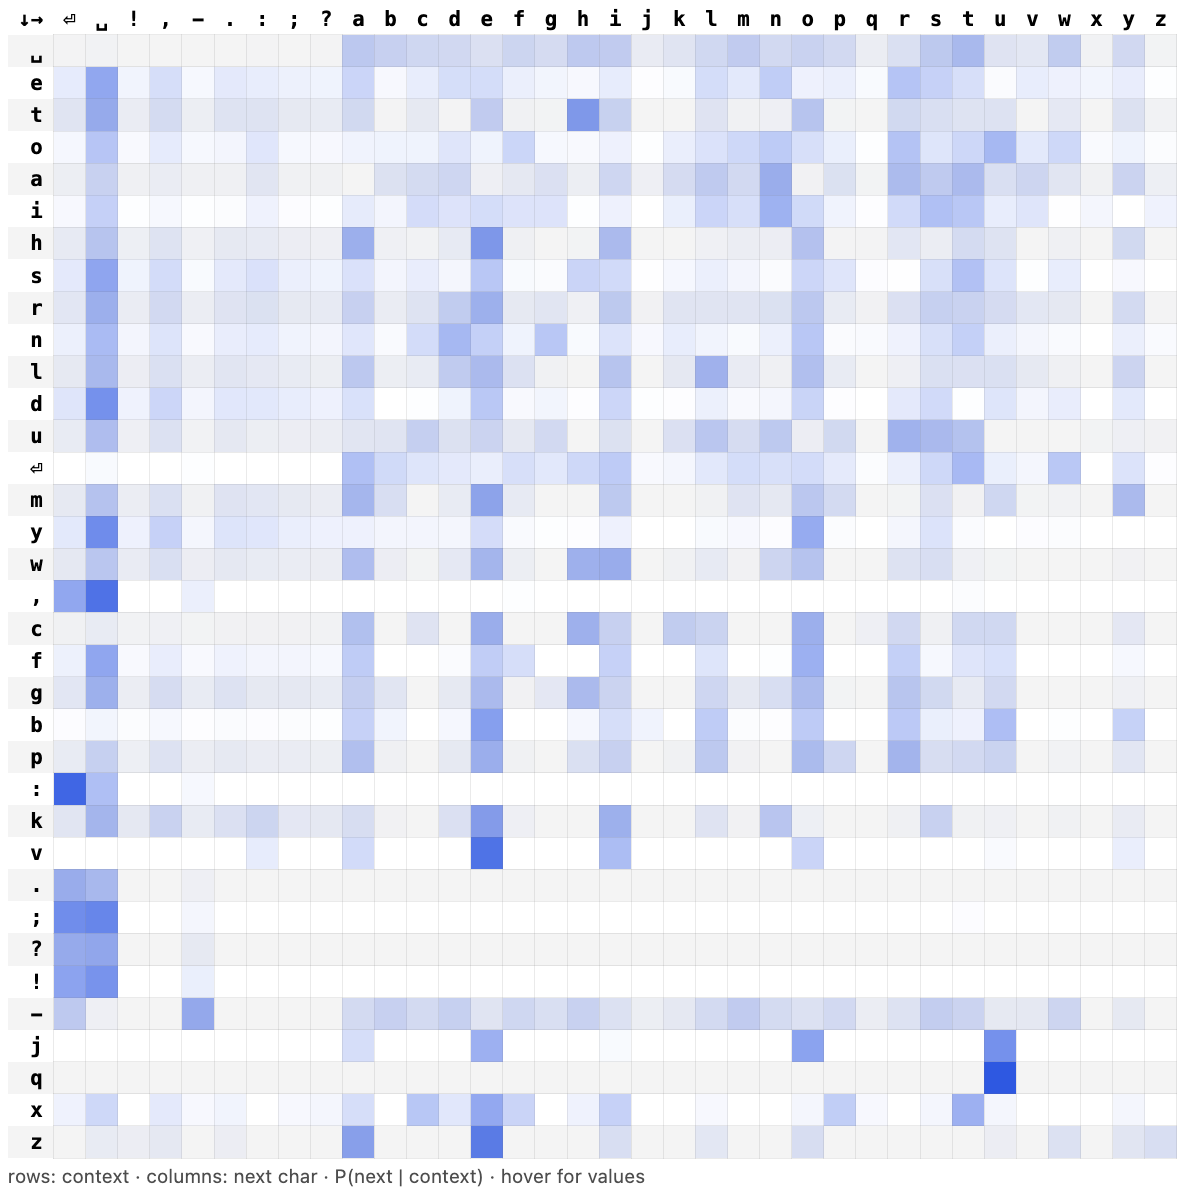
\includegraphics[width=.85\textwidth]{assets/uebergangsmatrix.png}
    \end{columns}
\end{frame}

\begin{frame}{N-Gram Modelle}{Sprachgenerierung}
    \vspace{-20pt} \centering
    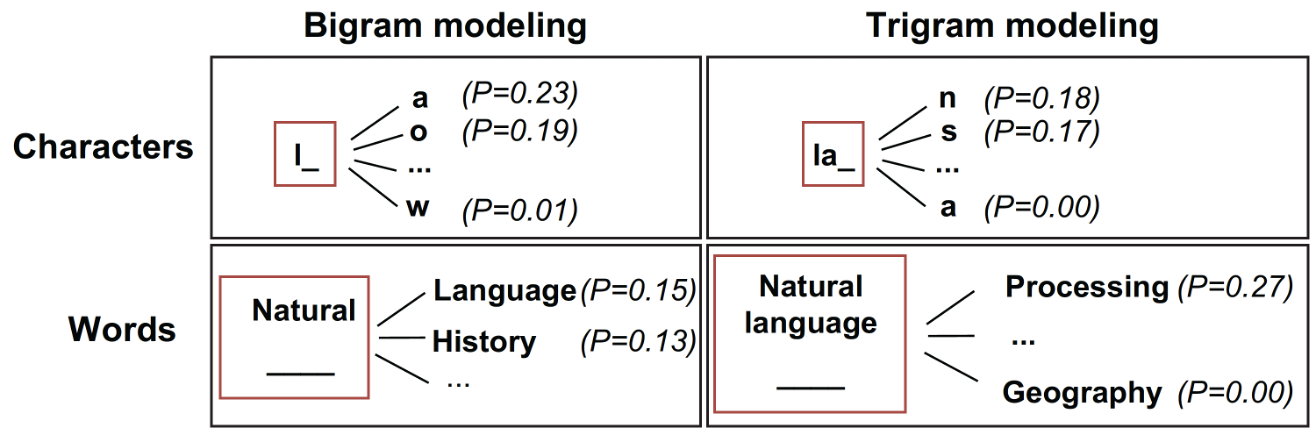
\includegraphics[width=.65\textwidth]{assets/n-gram-modeling.png}

    \smallskip \raggedright \footnotesize
    \textbf{Sampling:} Das Generieren des nächsten Tokens ist ein Zufallsexperiment. Im Gegensatz zu einem fairen Würfel (Gleichverteilung) ziehen wir hier aus einer \emph{gewichteten Verteilung}. Das Modell \enquote{würfelt} das nächste Zeichen, wobei Zeichen mit hoher relativer Häufigkeit eine entsprechend größere Trefferfläche auf unserem gedachten \enquote{Sprach-Würfel} haben.

    \framebib{kochmarGettingStartedNatural2022}
\end{frame}

\subsection{Skalierbarkeit \& Curse of Dimensionality}

\begin{frame}{Curse of Dimensionality}
    \begin{definition}[Curse of Dimensionality]
        \scriptsize
        Der \textbf{Curse of Dimensionality} veranschaulicht exponentielles Wachstum. Bei einem Vokabular der Größe $\lvert V\rvert$ gibt es für ein N-Gram Modell exakt $\lvert V\rvert^N$ mögliche Kombinationen (Ziehen mit Zurücklegen unter Beachtung der Reihenfolge).

        \smallskip\tiny\texttt{Kombinatorik $\cdot$ Exponentialfunktion}
    \end{definition}

    \begin{example}[Curse of Dimensionality]
        \scriptsize
        Für ein einfaches Bi-Gram auf Charakterebene ohne Sonderzeichen und Groß- und Kleinschreibung ergibt sich eine Matrix der Größe:
        \begin{equation*}
            \lvert V\rvert^N=26^2=676
        \end{equation*}

        Für ein modernes Sprachmodell wie GPT-4 liegt die Größe des Vokabulars bei 200.000. Bereits bei einem Bi-Gram würde sich damit eine Matrix der Größe
        \begin{equation*}
            \lvert V\rvert^N=200.000^2=4\times10^{10}
        \end{equation*}
        ergeben. Diese Matrizen sind \emph{schwachbesetzt}.
    \end{example}
\end{frame}

\begin{frame}{Curse of Dimensionality}
    \begin{columns}[onlytextwidth,c]
        \column{.39\textwidth} \footnotesize
        Spätestens ab der gestrichelten Linie treten \emph{theoretische} Sequenzen auf, die in den Daten nicht repräsentiert sind. Diese Kombinationen haben eine Übergangswahrscheinlichkeit von $0$; durch die multiplikative Verknüpfung ist dann die Wahrscheinlichkeit der gesamten Folge $0$!

        \smallskip Durch \emph{Laplace-Smoothing} werden kleine konstante Werte zu jeder möglichen Zelle hinzugefügt, um den vollständigen Verfall der Wahrscheinlichkeiten zu verhindern.

        \begin{equation*}
            P(r~\vert~q)=\frac{\texttt{Alte Anzahl (q $\rightarrow$ r)} + 1}{\texttt{Alte Zeilensumme q} + 26}
        \end{equation*}

        \column{.6\textwidth}
        \centering
        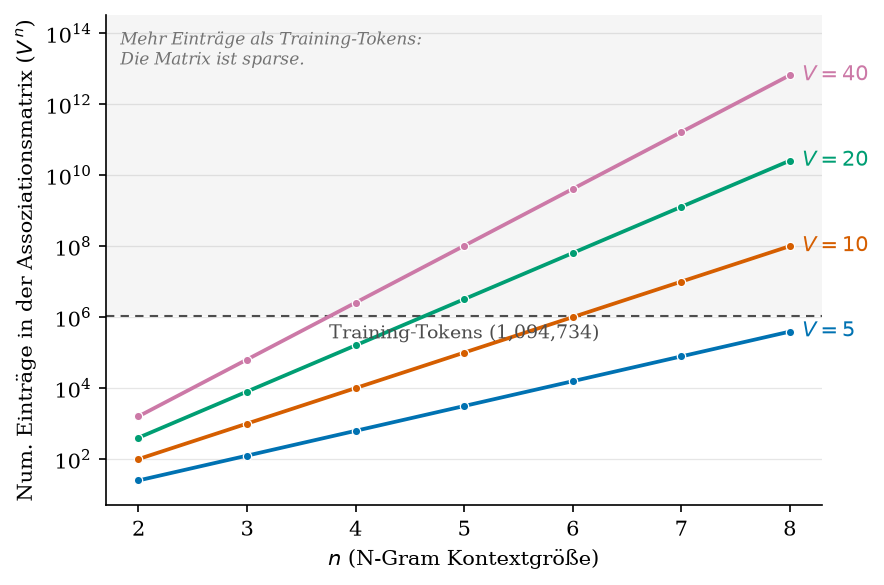
\includegraphics[width=\textwidth]{assets/matrix-scaling.png}
    \end{columns}
\end{frame}

\begin{frame}[c]{Gedächtnisverlust}
    Ein N-Gram Modell hat ein Kontextfenster (Gedächtnis) von $N-1$. Eine Frage wie:

    \smallskip \enquote{John und Mary sitzen am Tisch. Mit wem sitzt John am Tisch? \dots}

    \smallskip würden Sie vermutlich problemlos mit \enquote{Mary} beantworten. Ein N-Gram Modell geringer Ordnung hat an der Stelle jedoch leider wieder \enquote{vergessen}, dass es Mary jemals gab. N-Gram Sprachmodelle sind also nicht in der Lage, Informationen über längere Kontexte zu erhalten.
\end{frame}

%%%%%%%%%%%%%%%%% Vektorrepräsentationen %%%%%%%%%%%%%%%%%
\section{Vektorrepräsentationen}

\begin{frame}{Motivation}
    % TODO: Die Neuronalen Netze hier erwähnen too soon? Führen ja die neuronalen Sprachmodelle erst später ein...
    \begin{columns}[onlytextwidth,c]
        \column{.6\textwidth}
        \begin{itemize}
            \item Neuronale Netze verwenden dieselben Parameter, unabhängig vom Input
            \item Die Wahrscheinlichkeit einer Sequenz würde also durch die kombinierte Aktivierung verschiedener Parameter repräsentiert werden, anstelle durch eine exklusive Zelle in einer großen Matrix
            \item[$\rightarrow$] Das löst unser Skalierungsproblem (teilweise)

                \medskip
            \item Aber: Neuronale Netze brauchen reellwertige Eingaben, d.h. die \emph{diskreten} Token müssen \emph{vektorisiert} werden
        \end{itemize}

        \column{.39\textwidth}
        \centering
        \begin{tikzpicture}[
                x=1.3cm, y=0.75cm,
                neuron/.style={circle, draw=cogsysink, line width=0.6pt, minimum size=0.45cm, inner sep=0pt},
                edge/.style={draw=cogsysgrey777, line width=0.3pt},
            ]
            % Neuronen: Schicht/Anzahl/Farbe
            \foreach \layer/\n/\col in {0/3/ubblue!25, 1/4/cogsysexcursus, 2/4/cogsysexcursus, 3/2/ubgreen!40} {
                \foreach \i in {1,...,\n} {
                    \node[neuron, fill=\col] (N\layer-\i) at (\layer, {(\n+1)/2 - \i}) {};
                }
            }
            % Vollständige Verbindungen: Schicht/Anzahl/vorherige Schicht/deren Anzahl
            \foreach \layer/\n/\prev/\m in {1/4/0/3, 2/4/1/4, 3/2/2/4} {
                \foreach \i in {1,...,\n} {
                    \foreach \j in {1,...,\m} {
                        \draw[edge] (N\prev-\j) -- (N\layer-\i);
                    }
                }
            }
            % Beschriftungen
            \begin{scope}[font=\scriptsize, text=cogsysgrey555]
                \node at (0, -2.3) {Eingabe};
                \node at (1.5, -2.3) {Verdeckte Schichten};
                \node at (3, -2.3) {Ausgabe};
            \end{scope}
        \end{tikzpicture}

    \end{columns}
\end{frame}

% TODO: Bag-of-Words Ansätze? Sind aber Document-Reps, nicht für Tokens
% TODO: Oder: Wollen wir auch IR machen, oder bei der Sprachgenerierung bleiben?

\begin{frame}{Embeddings}{One-Hot Vektoren}
    \textbf{Idee:} Die Vektorrepräsentation hat die Größe $\lvert V\rvert$, wobei jedes Element im Vektor einem möglichen Token entspricht. Um ein Token zu repräsentieren, wird das entsprechende Element auf 1 gesetzt; alle anderen Elemente bleiben 0.

    \medskip
    \begin{itemize}
        \item Simpel

            \smallskip
        \item Hochdimensional (erinnere GPT-4, $\lvert V\rvert=200.000$)
        \item Per definition schwachbesetzt $\rightarrow$ ineffizient
        \item keine Semantik
    \end{itemize}
\end{frame}

\begin{frame}[excursus]{Abstandsmaße}{Euklidische Distanz}
    \begin{columns}[onlytextwidth,c]
        \column{.49\textwidth}
        \begin{equation*}
            d(p,q) = \sqrt{\sum_{i=1}^{n}(p_i-q_i)^2}
        \end{equation*}
        \begin{itemize}
            \item Für $n=2$ entspricht es dem Satz des Pythagoras
            \item Wenig aussagekräftig in höheren Dimensionen
        \end{itemize}

        \column{.5\textwidth}
        \centering
        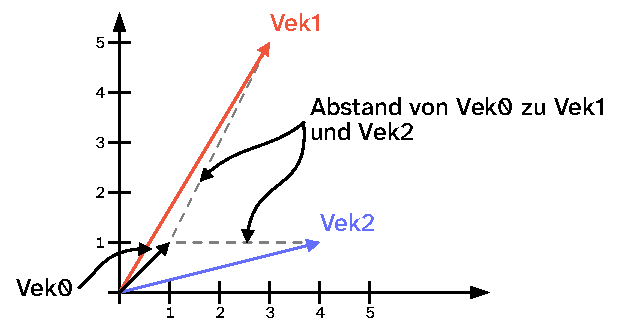
\includegraphics[width=\textwidth]{assets/euclidean.pdf}
    \end{columns}
\end{frame}

\begin{frame}[excursus]{Abstandsmaße}{Kosinusähnlichkeit}
    \begin{columns}[onlytextwidth,c]
        \column{.39\textwidth}
        \begin{equation*}
            S_C(p,q)=\frac{p~\cdot~q}{\lVert p\rVert~\lVert q\rVert}
        \end{equation*}
        \begin{itemize}
            \item Entspricht dem Winkel zwischen zwei Vektoren
            \item Robust in höheren Dimensionen
        \end{itemize}

        \column{.6\textwidth}
        \centering
        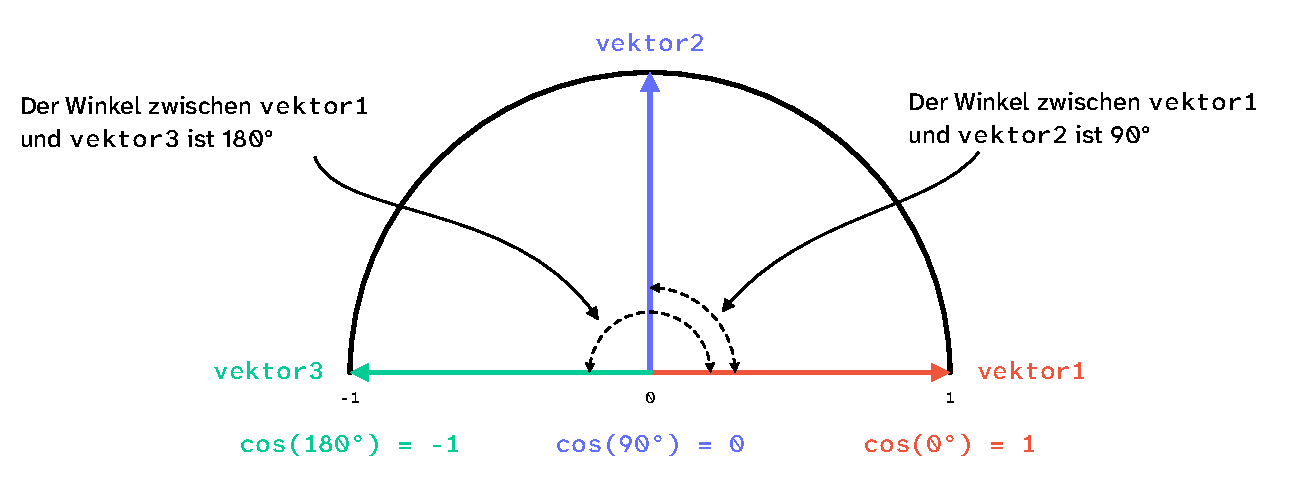
\includegraphics[width=\textwidth]{assets/cosine.pdf}
    \end{columns}
\end{frame}

\begin{frame}{Embeddings}{Word2Vec}
    \begin{itemize}
        \item Interessante Beobachtung: Wörter mit ähnlichen Bedeutungen tauchen in ähnlichen Kontexten auf
        \item Wörter werden Vektoren in $\mathbb{R}^N$ bei \emph{relativ} großen $N~\in~[500,2000]$ zugewiesen
        \item Diese Zuweisung (\emph{Projektion}) wird optimiert, sodass $d(w_1,w_2)~\sim~d(c_1,c_2)$, wobei $c_i$ der lexikalische Kontext von $w_i$ ist
        \item Semantisch ähnliche Wörter tauchen in ähnlichen Kontexten auf, d.h. wenn die Kontexte im Vektorraum nah beieinander liegen, sollten auch die Wörter nah beieinander liegen
    \end{itemize}
\end{frame}

\begin{frame}{Embeddings}{Word2Vec}
    \begin{columns}[onlytextwidth,c]
        \column{.54\textwidth}
        So können implizit Beziehungen zwischen Wörtern gelernt werden
        \begin{align*}
            &\operatorname{vec}(\textit{Berlin})~-~\operatorname{vec}(\textit{Germany})~+~\operatorname{vec}(\textit{France}) \\ &=~?
        \end{align*}

        \column{.45\textwidth}
        \centering
        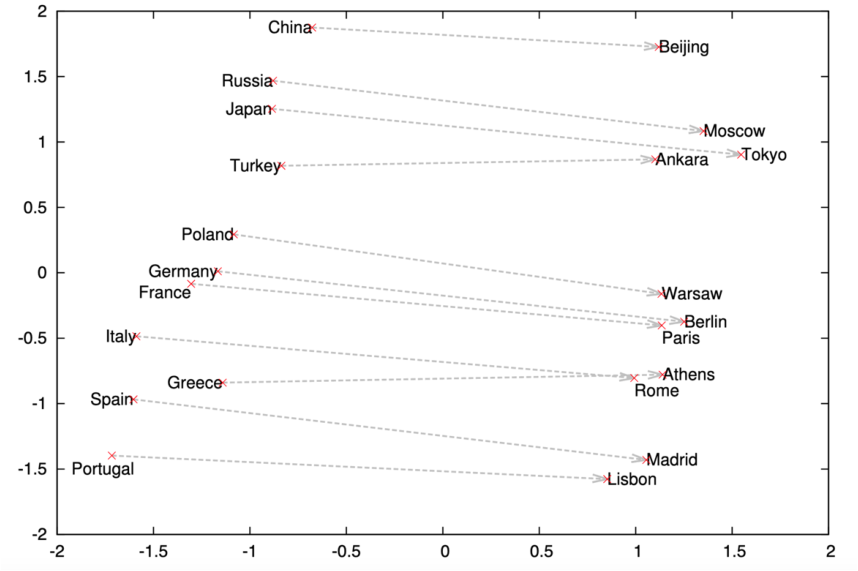
\includegraphics[width=\textwidth]{assets/capitals.pdf}
    \end{columns}

    \framebib{mikolovDistributedRepresentationsWords2013}
\end{frame}

\begin{frame}{Embeddings}
    \begin{itemize}
        \item Word-Embeddings können zum Beispiel für \emph{Information Retrieval} verwendet werden, ohne dass per se ein Sprachmodell angewendet werde muss (z.B. in eigentlich jeder digitalen Schlagwortsuche, oder um in RAG-Systemen Sprachmodelle mit dem richtigen Kontext zu versorgen)
        \item Word-Embeddings erleichtern das Training vom \emph{eigentlichen} Sprachmodell (einfacheres Trainingsziel, wiederverwenden von bestehenden Modellen), oder werden effektiv beim Lernen von großen Modellen mitgelernt
    \end{itemize}
\end{frame}

%%%%%%%%%%%%%%%%% Neuronale Sprachmodelle %%%%%%%%%%%%%%%%%
\section{Neuronale Sprachmodelle}

\begin{frame}{Definition}
    \begin{definition}[Neuronales Sprachmodell]
        $f$ sei ein neuronales Netz, parametrisiert durch $\theta$, und $w_1^T$ eine Wortfolge der Länge $T$. Dann ist
        \begin{equation*}
            \hat{P}(w_T~\vert~w_1^{T-1})=f(w_1^{T-1},\theta)
        \end{equation*}
        ein \textbf{neuronales Sprachmodell}.
    \end{definition}
\end{frame}

\subsection{Attention}

\begin{frame}{Attention}{Motivation}
    \begin{itemize}
        \item Frühe neuronale Sprachmodelle konnten zwar Informationen über längere Sequenzen verarbeiten als N-Gram Modelle, litten aber unter einem graduellen Verlust von Kontextinformationen
        \item Solche \emph{Rekurrente Neuronale Netze} geben Informationen aus vergangenen Netzwerkdurchläufen \emph{direkt verkettet} an spätere Durchläufe weiter
        \item In solchen Netzwerken ist es besonders schwierig, Informationen aufgrund ihrer \emph{Relevanz}, anstelle ihrer Position, zu verarbeiten und über längere Sequenzen hinweg zu priorisieren
    \end{itemize}
\end{frame}

\begin{frame}{Attention}
    % TODO: Braucht die Slide Visualization (insb. für den ersten Stichpunkt)?
    \begin{columns}[onlytextwidth,T]
        \column{.55\textwidth} \footnotesize
        \begin{itemize}
            \item Aus jedem Token in einer Folge von Token-Embeddings wird mit gelernten Projektionen ein \emph{Query}, \emph{Key}, und \emph{Value} Vektor erstellt
        \end{itemize}

        \begin{equation*}
            \operatorname{Attention}(Q,K,V)=\operatorname{softmax}\left(\frac{QK^T}{\sqrt{d_k}}\right)V
        \end{equation*}

        \begin{itemize}
            \item Die $\operatorname{softmax}$-Verteilung sorgt dafür, das je nach Höhe des Skalarproduktes zwischen \emph{Query} und \emph{Key} ein entsprechender Anteil des zum \emph{Key} gehörenden \emph{Value} in das Ergebnis einfließt (der {\tiny$\frac{1}{\sqrt{d_k}}$} Skalar sorgt für eine stabile Verteilung auch bei hohen Dimensionen)
            \item Nach einer Attention-Schicht beinhaltet die Sequenz also nicht nur Informationen zur Semantik der einzelnen Tokens (durch Embeddings), sondern auch Informationen zu deren Kontext
        \end{itemize}

        \column{.4\textwidth}
        \begin{excursusblock}{Hashmaps} \footnotesize
            Hashmaps, oder Hash-Tabellen, sind eine beliebte Datenstruktur, die flexiblen und äußerst schnellen Zugriff auf ihre gespeicherten Daten bieten (Komplexität $O(1)$).

            \medskip
            In der Anwendung wird über Schlüssel (\emph{Keys}) auf die dahinter liegenden Werte (\emph{Values}) zugegriffen.

            \medskip
            Eine Anfrage (\emph{Query}) in dieser Analogie würde nicht perfekt auf einen Schlüssel passen, sondern müsste zunächst bei allen Schlüssel abgleichen, wie gut sie zur Anfrage passen.
        \end{excursusblock}
    \end{columns}
\end{frame}

\begin{frame}[excursus]{Transformer}
    \begin{columns}[onlytextwidth,c]
        \column{.6\textwidth} \small
        \begin{itemize}
            \item Die Abbildung rechts zeigt einen \enquote{\emph{Decoder-Only-Transformer}}, die Standard-Architektur für moderne große Sprachmodelle
                % TODO: "Additiver Faktor", kann man das so sagen? :D
            \item \enquote{+ Position}: Transformer nutzen keine Rekurrenz (d.h. weitergabe von vorherigen Netzwerkläufen), und die reinen Matrizenmultiplikationen aus den Schichten des Netzwerks sind invariant zur Reihenfolge der Tokens. Deshalb benötigen die Token-Embeddings einen additiven Faktor, aus dem die Reihenfolge der Tokens nachvollziehbar wird.
            \item Am Ende wird eine Softmax-Verteilung über das Vokabular aufgespannt. \\
                $\rightarrow$ Die Auswahl des nächsten Tokens entspricht also effektiv einer \emph{Klassifikation}.
        \end{itemize}

        \column{.4\textwidth}
        \centering
        \begin{tikzpicture}[
                font=\scriptsize,
                layer/.style={draw=cogsysink, line width=0.6pt, rounded corners=2pt, minimum width=3.4cm, minimum height=0.42cm, inner sep=2pt, align=center},
                flow/.style={-latex, draw=cogsysink, line width=0.6pt},
                res/.style={-latex, draw=cogsysgrey777, line width=0.5pt, rounded corners=3pt},
            ]
            % Schichten (von unten nach oben)
            \node[text=cogsysgrey555]      (in)   at (0, 0)    {Eingabe-Token $w_1, \dots, w_t$};
            \node[layer, fill=ubyellow!35] (emb)  at (0, 0.6)  {Token-Embedding + Position};
            \node[layer, fill=ubblue!25]   (att)  at (0, 1.45) {Masked Self-Attention};
            \node[layer, fill=white]       (an1)  at (0, 2.05) {Add \& Norm};
            \node[layer, fill=ubgreen!40]  (ffn)  at (0, 2.75) {Feed-Forward-Netz};
            \node[layer, fill=white]       (an2)  at (0, 3.35) {Add \& Norm};
            \node[layer, fill=ubred!25]    (out)  at (0, 4.15) {Linear + Softmax};
            \node[text=cogsysgrey555]      (pred) at (0, 4.75) {$\hat{P}(w_{t+1}~\vert~w_1, \dots, w_t)$};

            % Hauptpfad
            \foreach \a/\b in {in/emb, emb/att, att/an1, an1/ffn, ffn/an2, an2/out, out/pred} {
                \draw[flow] (\a) -- (\b);
            }

            % Residualverbindungen (Umgehung von Attention bzw. Feed-Forward)
            \draw[res] ([yshift=-0.18cm]att.south) -- ++(1.95, 0) |- (an1.east);
            \draw[res] ([yshift=-0.14cm]ffn.south) -- ++(1.95, 0) |- (an2.east);

            % Transformer-Block (N-mal hintereinander)
            \draw[cogsysgrey555, dashed, rounded corners=4pt]
            ([xshift=-0.15cm, yshift=-0.3cm]att.south west) rectangle ([xshift=0.35cm, yshift=0.12cm]an2.north east);
            \node[text=cogsysgrey555, anchor=east] at ([xshift=-0.2cm, yshift=-0.35cm]an1.north west) {$N\times$};
        \end{tikzpicture}
    \end{columns}
\end{frame}

\subsection{Autoregression}

\begin{frame}[essential]{Sprachgenerierung/Autoregression}
    \small
    \textbf{Sprachgenerierung mit neuronalen Sprachmodellen ist Klassifikation.}
    \begin{itemize}
        \item Das Modell gibt eine Wahrscheinlichkeitsverteilung über das Vokabular aus (d.h. \enquote{Wie wahrscheinlich ist es, dass \emph{dieses} Token das nächste in der Sequenz ist?})
        \item Das nächste Token wird entweder deterministisch gewählt, indem das wahrscheinlichste Token gewählt wird, oder indem gewichtet aus der Verteilung \enquote{gezogen} wird.
    \end{itemize}

    \begin{definition}[Autoregression] \footnotesize
        \begin{itemize}
            \item Transformer generieren Text Schritt-für-Schritt
            \item In jedem Schritt wird das generierte Token zur Kontextfolge hinzugefügt, um die Generierung des nächsten Tokens zu beeinflussen \\
                $\rightarrow$ \textbf{Autoregression}
            \item Jede Position kann sich bei der Berechnung der \emph{Attention} nur auf vorherige Positionen in der Folge beziehen (\emph{kausale Maske})
        \end{itemize}
    \end{definition}
\end{frame}

\subsection{Dialogsysteme}

\begin{frame}[c]
    \vspace{40pt}
    \huge
    \textbf{Was braucht ein Sprachmodell, damit es zum Chat-Modell wird?}
    % - Gedächtnis
    % - Antworten, anstatt Text fortzusetzen
    % - Schnell
    % -> Erklärt, warum erst mit Transformern Chatbots richtig gut wurden, und nicht schon vorher
\end{frame}

\begin{frame}{Dialogsysteme}{Vom Sprachmodell zum Chat-Interface}

\end{frame}

%%%%%%%%%%%%%%%%% Abschluss %%%%%%%%%%%%%%%%%
\section[noframe]{Abschluss}

\begin{frame}{Zusammenfassung}

\end{frame}

\begin{frame}{Über Uns}

\end{frame}

%%%%%%%%%%%%%%%%% Backup Slides %%%%%%%%%%%%%%%%%
\section*{Backup Slides}

% Herleitung 1/root(dk)
\begin{frame}{Skalierte Dot-Product-Attention}{Herleitung $\frac{1}{\sqrt{d_K}}$}
    Annahme: $Q$ und $K$ sind unabhängig, mit $\mu=0$ und $\sigma^2=1$
    \begin{align*}
        \operatorname{Var}(S_{ij})
        &= \mathbb{E}\Big[\Big(\textstyle\sum_{l} Q_{il}K_{jl}\Big)^2\Big]
        && \text{(da } \mathbb{E}[S_{ij}] = 0\text{)} \\
        &= \textstyle\sum_{l}\mathbb{E}[Q_{il}^2]\,\mathbb{E}[K_{jl}^2]
        + \sum_{l\neq r}\underbrace{\mathbb{E}[Q_{il}]\mathbb{E}[K_{jl}]\mathbb{E}[Q_{ir}]\mathbb{E}[K_{jr}]}_{=0}
        && \text{(statistische Unabhängigkeit)} \\
        &= \textstyle\sum_{l=1}^{d_k} 1 \cdot 1 = d_k
    \end{align*}
\end{frame}

\end{document}
